%%%%%%%%%%%%%%%%%%%%%%%%%%%%%%%%%%%%%%%%%
% Tufte-Style Book (Minimal Template)
% LaTeX Template
% Version 1.0 (5/1/13)
%
% This template has been downloaded from:
% http://www.LaTeXTemplates.com
%
% License:
% CC BY-NC-SA 3.0 (http://creativecommons.org/licenses/by-nc-sa/3.0/)
%
% IMPORTANT NOTE:
% In addition to running BibTeX to compile the reference list from the .bib
% file, you will need to run MakeIndex to compile the index at the end of the
% document.
%
%%%%%%%%%%%%%%%%%%%%%%%%%%%%%%%%%%%%%%%%%
%%% LaTeX-command: "latex -shell-escape"
%----------------------------------------------------------------------------------------
%	PACKAGES AND OTHER DOCUMENT CONFIGURATIONS
%----------------------------------------------------------------------------------------

\documentclass{tufte-book} % Use the tufte-book class which in turn uses the tufte-common class

\hypersetup{colorlinks} % Comment this line if you don't wish to have colored links

\usepackage{microtype} % Improves character and word spacing
\usepackage{listings}
\usepackage{lipsum} % Inserts dummy text
\usepackage{amsmath}
\usepackage{booktabs} % Better horizontal rules in tables
\usepackage{minted}
\usemintedstyle{borland}
%\usepackage{xcolor}
\usepackage{graphicx} % Needed to insert images into the document
\graphicspath{{graphics/}} % Sets the default location of pictures
\setkeys{Gin}{width=\linewidth,totalheight=\textheight,keepaspectratio} % Improves figure scaling

\usepackage{fancyvrb} % Allows customization of verbatim environments
\fvset{fontsize=\normalsize} % The font size of all verbatim text can be changed here

\newcommand{\hangp}[1]{\makebox[0pt][r]{(}#1\makebox[0pt][l]{)}} % New command to create parentheses around text in tables which take up no horizontal space - this improves column spacing
\newcommand{\hangstar}{\makebox[0pt][l]{*}} % New command to create asterisks in tables which take up no horizontal space - this improves column spacing
\usepackage{subfig}
\usepackage{xspace} % Used for printing a trailing space better than using a tilde (~) using the \xspace command
\usepackage{hyperref}
\newcommand{\monthyear}{\ifcase\month\or January\or February\or March\or April\or May\or June\or July\or August\or September\or October\or November\or December\fi\space\number\year} % A command to print the current month and year

\newcommand{\openepigraph}[2]{ % This block sets up a command for printing an epigraph with 2 arguments - the quote and the author
\begin{fullwidth}
\sffamily\large
\begin{doublespace}
\noindent\allcaps{#1}\\ % The quote
\noindent\allcaps{#2} % The author
\end{doublespace}
\end{fullwidth}
}

\newcommand{\blankpage}{\newpage\hbox{}\thispagestyle{empty}\newpage} % Command to insert a blank page
\newcommand{\Li}{\textit{LIGGGHTS}}
\newcommand{\La}{\textit{LAMMPS}}

\newcommand{\TL}{Tufte-\LaTeX\xspace}
\usepackage{makeidx} % Used to generate the index
\makeindex % Generate the index which is printed at the end of the document

%----------------------------------------------------------------------------------------
%	BOOK META-INFORMATION
%----------------------------------------------------------------------------------------

\title{Discrete Element Method} % Title of the book

\author{Siddharth Kanungo} % Author

\publisher{Ryan Gosselin, Nicolas Abatzoglou} % Publisher

%----------------------------------------------------------------------------------------

\begin{document}

\frontmatter

%----------------------------------------------------------------------------------------
%	EPIGRAPH
%----------------------------------------------------------------------------------------

\thispagestyle{empty}
\openepigraph{ }{Buddha, {\itshape Dhammapada}}
\vfill
% \openepigraph{Quotation 2}{Author}
% \vfill
% \openepigraph{Quotation 3}{Author}

%----------------------------------------------------------------------------------------

\maketitle % Print the title page

%----------------------------------------------------------------------------------------
%	COPYRIGHT PAGE
%----------------------------------------------------------------------------------------

\newpage
\begin{fullwidth}
~\vfill
\thispagestyle{empty}
\setlength{\parindent}{0pt}
\setlength{\parskip}{\baselineskip}
\thanklessauthor

\par\smallcaps{Under the guidance of \thanklesspublisher}

\par \smallcaps{MITACS Globalink Research Internship}

\par\textit{Submitted  \monthyear}
\end{fullwidth}

%----------------------------------------------------------------------------------------

\tableofcontents % Print the table of contents

%----------------------------------------------------------------------------------------

\listoffigures % Print a list of figures

%----------------------------------------------------------------------------------------

\listoftables % Print a list of tables

%----------------------------------------------------------------------------------------
%	DEDICATION PAGE
%----------------------------------------------------------------------------------------

\cleardoublepage
~\vfill
\begin{doublespace}
\noindent\fontsize{18}{22}\selectfont\itshape
\nohyphenation
To my rational brain, for always being there for me, despite all the shaky evidences pointing otherwise. 
\end{doublespace}
\vfill
\vfill

%----------------------------------------------------------------------------------------
%	INTRODUCTION
%----------------------------------------------------------------------------------------

\cleardoublepage
\chapter{Acknowledgement} % The asterisk leaves out this chapter from the table of contents
\label{ch:0}
 \index{acknowledgement}

    \newthought{This Documentation} is a part of the project that I
    worked on during the summer of 2015 at the PAT-Pfizer Chair in
    Universit\'e  d\'e  Sherbrooke. This document wouldn't have been
    possible without the guidance of Prof. Ryan Gosselin and
    Prof. Nicolas Abatzoglou. 

    \newthought{I would also} like to also like to thank all the Lab Members of the Research Group, who helped me generously during my internship and graciously welcomed me into their part of the life.

   \newthought{A special thanks} to Pedro Dura\'o, Philippe Kikongi, Himmat Dalvi, Francis Lavois, Ounaima  and 

   \newthought{ I would also like} to thank all the people I met during the internship, who helped me settle in and feel welcome at the same time. At last I would like to thanks MITACS for funding this incredible journey.
    
    \newthought{This document was} submitted much late than it was supposed, even though it was almost completed very early. I would sincerely apologize for that. 

   

   \newthought{ Siddharth Kanungo}
    
    
 

%------------------------------------------------

%----------------------------------------------------------------------------------------

\mainmatter

%----------------------------------------------------------------------------------------
%	CHAPTER 1
%----------------------------------------------------------------------------------------

\chapter{Working With Ubuntu}
\label{ch:1}

%------------------------------------------------

\section{Introduction}

\begin{fullwidth}
  It is very essential that one should learn about the operating system that one would be working with while using \textsc{\Li}. Unlike Windows, which offers the least learning curve to adequately use the Machine, in Linux-based Operating systems, there is a quite a bit of learning curve and for someone who has never been exposed to Unix based system, this can seem overwhelming. However, in order to work with \textsc{LIGGGHTS}, we will use an operating System called \emph{Ubuntu}, which was designed keeping in mind the ease of using Windows in the first place. Therefore, apart from a few basic commands, which will become intuitive with progressive use, there are not many commmands that one must learn to use \textsc{\Li}. The following section will give introuction to the history of Ubuntu, Linux and basics of computing in general. The reader may skip and proceed directly to subsequent sections, without any loss of continuity.
\end{fullwidth}
 \index{Ubuntu}
\subsection{Operating Systems}

\newthought{An operating system} is a piece of software you can install on a computer whose purpose is to manage the hardware so that other programs you use don't have to do it. That means programmers of Microsoft Word do not have to worry about what kinds of graphics card you have in order to display letters on your screen since the operating system takes care of that for it. This makes it easier for programmers to make software that works together.\sidenote{This has edited from the discussion present \href{https://www.reddit.com/r/explainlikeimfive/comments/16digd/eli5_the_relationship_between_unix_linux_and/c7v0xg6}{here} } 
\index{Operating System}
\emph{Linux, Unix, and Ubuntu} are all operating systems, however there are subtle differences between them. For example Ubuntu is a kind of Linux, and Linux is basically UNIX rewritten from scratch.

\newthought{A kernel} is the \textit{core} part of an operating system. Microsoft's Windows has a kernel as well, albeit obviously a different one from UNIX and Linux. The kernel does all the very low-level dirty work of the operating system like decide how files are stored to your disk or providing an interface to other programs that allow them to output sound without having to write new code for each type of sound card out there. Aside from a kernel, other things are often included with an operating system and are considered part of the package. For example, Windows comes with a graphics interface that is not really separable from it whereas Linux can run without a graphical interface just fine.

\subsection{Unix \& Linux}
\newthought{Unix is an operating system} that was originally created at Bell Labs in the late 1960s/early '70s. In the '70s and '80s it became very popular, and various derivative versions were made - some by commercial companies.


In the early 1990s, Linus Torvalds created \textit{Linux} while he was at university in Helsinki. Linux isn't based on Unix, but is more like a clone or remake. So to the user it mostly behaves the same as Unix, although technically it isn't derived from Unix. Linus wanted there to be a free version of Unix that could be used on PCs (at the time most versions of Unix cost money and required expensive computers). It became very popular, other people contributed code to it and it is now one of the most-used operating systems in the world.
\textit{Linux} itself is just a kernel. As explained in the previous section, the kernel is the core of the operating system - it "sets the stage" on which everything else runs. The complete system is often referred to as "Linux", but it's actually Linux plus a whole load of different pieces of software from different projects.
There are many different \textsc{Linux distributions (or distros)}. A \textsc{distro} takes all of these different components and assembles them into a complete system that you can install on your computer. Although the end result is usually largely the same, different distros do things in slightly different ways. Ubuntu is one example of a distro. Others would be Debian, Fedora, Gentoo, etc.

\subsection[Ubuntu]{The Ubuntu Story}

\newthought{Ubuntu is an ancient African word } meaning \textsc{humanity to others}. It also means \emph{I am what I am because of who we all are}. The Ubuntu operating system brings the spirit of Ubuntu to the world of computers.\sidenote{For more information on Ubuntu, the reader can visit \href{http://www.ubuntu.com/about/about-ubuntu}{here}.}

\textbf{When did it all began?}
\emph{Linux} was already established as an enterprise server platform in 2004, but free software was not a part of everyday life for most computer users. That is why \textit{Mark Shuttleworth} gathered a small team of developers from one of the most established Linux projects Debian and set out to create an easy-to-use Linux desktop:\textbf{ Ubuntu}.The vision for Ubuntu is part social and part economic: free software, available to everybody on the same terms, and funded through a portfolio of services provided by Canonical.
\index{Unix}
\index{Linux}
\index{Kernal}
\subsection[Open Source]{Open Source and Free Software }

\newthought{Open Source Movement and Free Software movement}\sidenote{For more information on philosophy of Ubuntu, the reader can read the philosophy of \href{http://www.ubuntu.com/about/about-ubuntu/our-philosophy}{Ubuntu}}both stem from the belief that software is a creative tool and it should be always available to each and every member of society to tinker with and expand on. Keeping in mind, Ubuntu meets the goal of free and open source software. 

\newthought{There is } a distinct design philosophy when someone from Windows \sidenote {There is an excellent write up on the philosophy of working in an Windows Environment to that of Linux Environment. It was written primarily for users who were \href{https://help.ubuntu.com/community/SwitchingToUbuntu/FromWindows/Philosophy}{\textsc{switching from Windows to Linux} }for the first time. It is highly recommended to give it a read} leaves its convienient shell to work in Linux-based environment starts to notice. These maybe, the subtle changes that one may notice in the working around the \textsc{operating system }. Although, these are primary essence of the user about the way he/she treats the work environment, sometimes it is worth the investment to understand why something is the way it has turned out be.

\newthought{I hope } that this short introduction will help the user to understand the key points of emergence of Linux as an alternative and therefore make the learning, a different and fun experience altogether.
%------------------------------------------------

\section{Terminal}
\begin{fullwidth}
The terminal is an interface in which you can type and execute text based commands.It can be much faster to complete some tasks using a Terminal than with graphical applications and menus. Another benefit is allowing access to many more commands and scripts. A common terminal task of installing an application can be achieved within a single command, compared to navigating through the Software Centre or Synaptic Manager. \sidenote{This has been taken from discussion \href{http://askubuntu.com/questions/38162/what-is-a-terminal-and-how-do-i-open-and-use-it}{here} }
\end{fullwidth}
\subsection{Getting into the Terminal}
\index{Terminal}
\newthought{There are two} ways to to get into terminal.
\begin{itemize}
\item Click on the Dash ( Windows Key/ Super Key)
\item Type terminal and wait for it find the application
\item Click on Terminal to access the Terminal. 
\end{itemize}

Alternatively, the terminal can also be accessed by using the shortcut
\begin{minted}{bash}
  CTRL + ALT + t
\end{minted}

\begin{figure*}[p]\index{opening terminal}
  \fbox{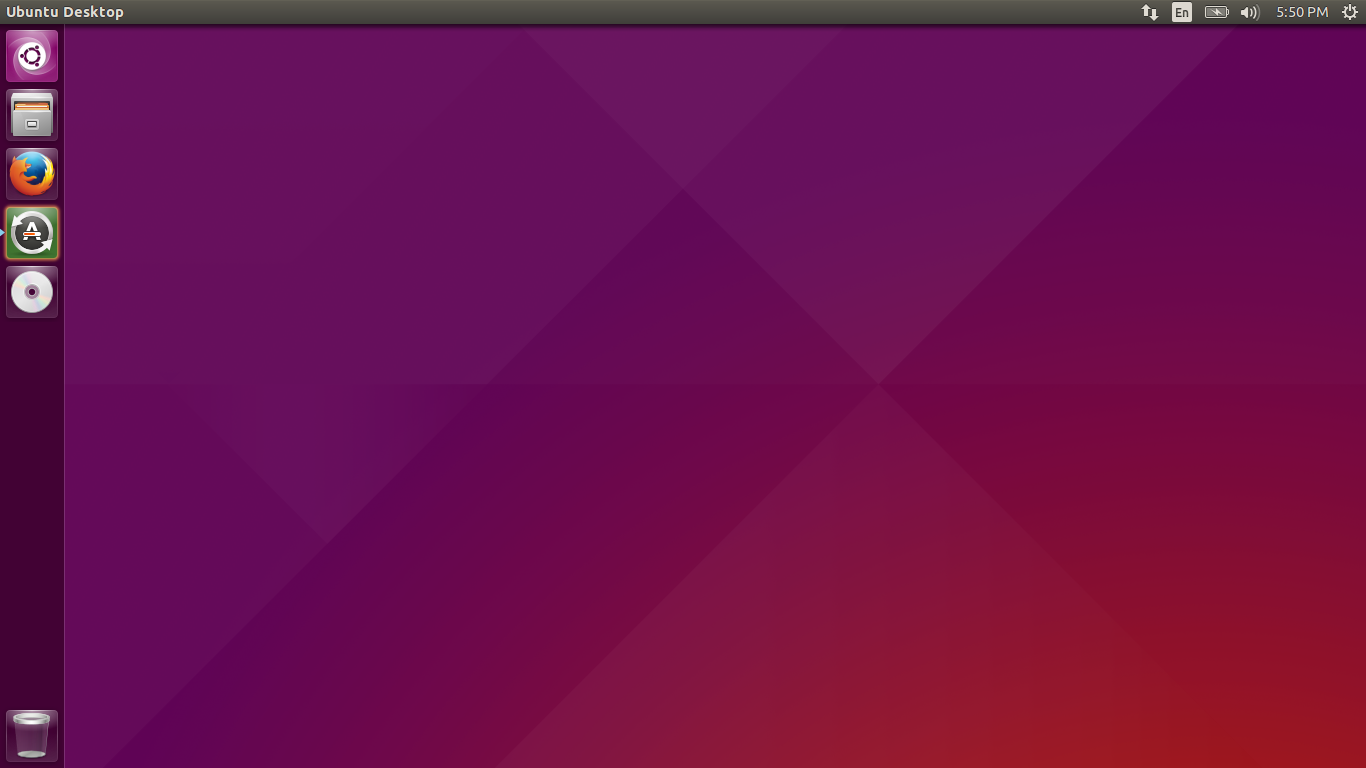
\includegraphics{graphics/Ubuntu_Desktop.png}}
  
 \vspace{\baselineskip}
\fbox{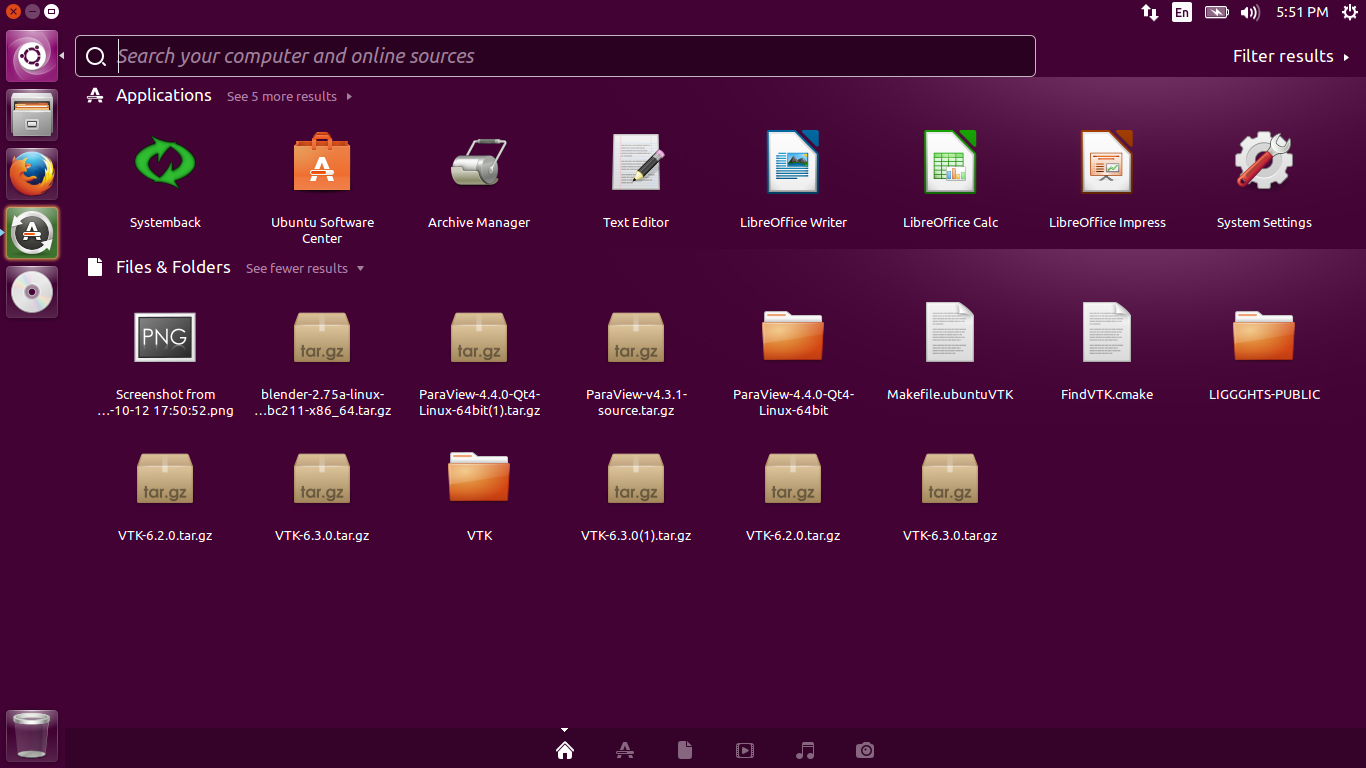
\includegraphics{graphics/Dash.png}}
%\caption[Dash]{}
  \caption[Appearance of Ubuntu Desktop]{\emph{Side-bar} is similar to start-menu of \textsc{Windows}. \emph{Dash} or start menu if you may call, gives access to the list of applications and settings installed the OS}

\end{figure*}


\begin{figure*}[p]\index{opening terminal}
\fbox{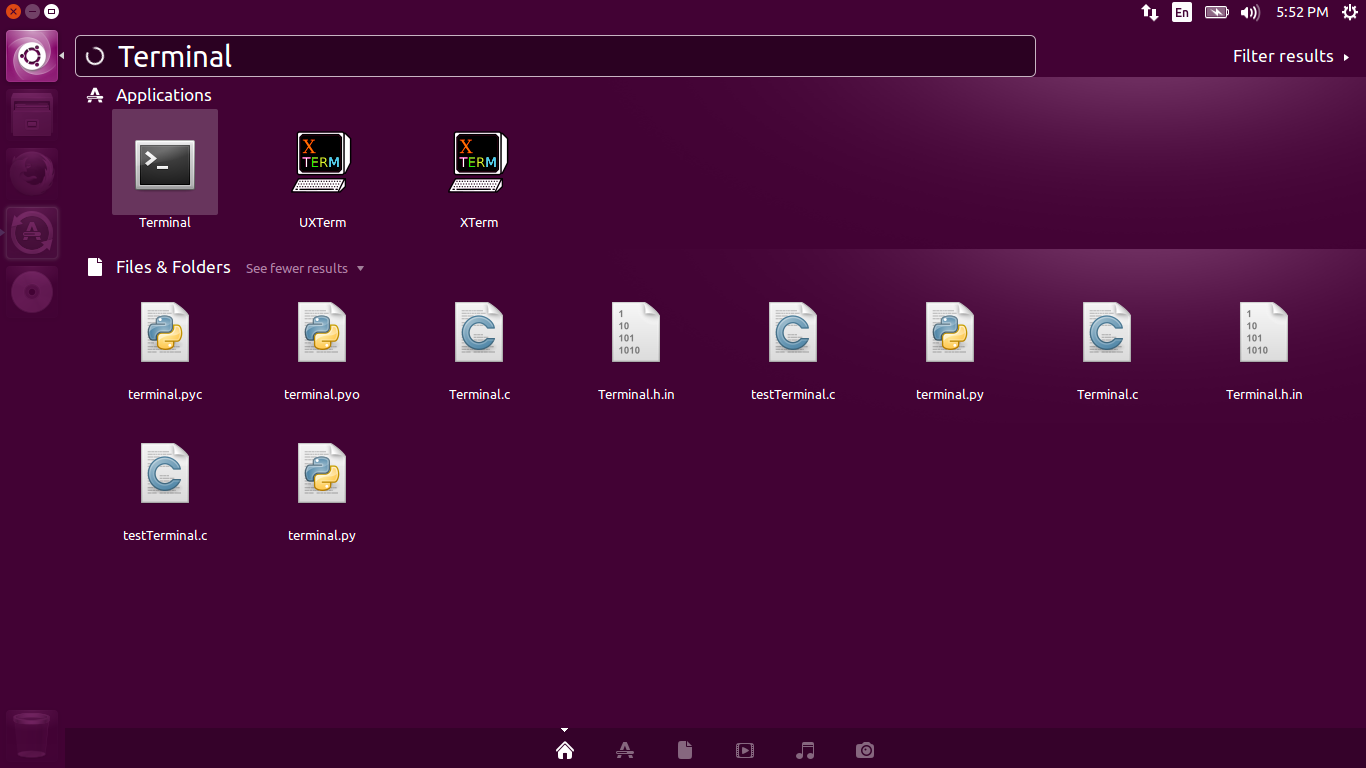
\includegraphics{graphics/Typing_Terminal.png}}
\\\vspace{\baselineskip}
\fbox{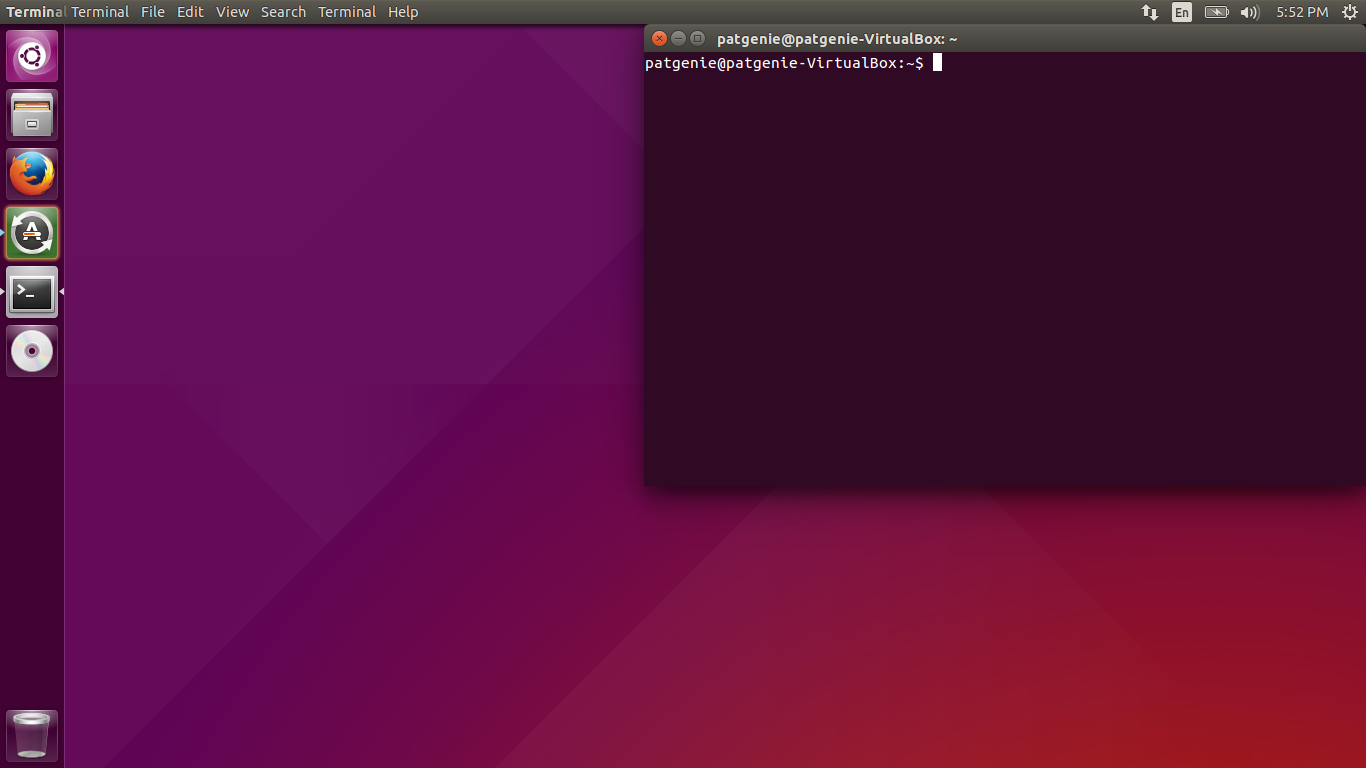
\includegraphics{graphics/Terminal.png}}
\caption{In the \emph{Dash}, type \emph{Terminal} and click on the Terminal Icon that appears. The terminal windows is shown in the above figure.}
\end{figure*}





\subsection{Common Commands}

\begin{fullwidth}
  The number of useful commands in \textsc{Ubuntu} while working with \Li is very limited. Therefore it is advisable to learn all the commands for better productivity and speeder navigation around the OS. It is also advisable to try each command in the shell for better and quick understanding. 
\end{fullwidth}

\begin{table*}[center]
  \centering
  \begin{tabular}{ll}
    \toprule
    Command & Usage \\
    \midrule
    cd .. & change directory and goes one folder up \\
    cd \textit{<foldername>} & change directory and go the specified folder \\
    cd \textit{<folderName1>/<folderName2>} & change directory and goto the specified folderName2 which is in folderName1 \\
    cd \textit{../<folderName>} & change directory and go one folder up and go to the specified folderName \\
    ls & List all files and folders \\
    ls \textit{-a} & List all files and folders including the hidden folders \\
    pwd & Find out the location of current directory \\
    
    \bottomrule
  \caption{Commonly Used Commands}
     
  \end{tabular}
  \label{command0}

\end{table*}


\subsection{Understanding filestructure of Ubuntu}
\newthought{The filesystem of Ubuntu} is somewhat different from that of Windows. Ubuntu (like all UNIX-like systems) organizes files in a hierarchical tree, where relationships are thought of in teams of children and parent.\sidenote{\href{http://www.howtogeek.com/117435/htg-explains-the-linux-directory-structure-explained/}{HowToGeek} has also a brief article about understanding the filestructure.} Directories can contain other directories as well as regular files, which are the "leaves" of the tree. Any element of the tree can be references by a path name; an absolute path name starts with the character / (identifying the root directory, which contains all other directories and files), then every child directory that must be traversed to reach the element is listed, each separated by a / sign.\sidenote{To understand more, visit this \href{https://help.ubuntu.com/community/LinuxFilesystemTreeOverview}{page}}


\subsection[Copy, Paste, Delete]{Copying, Paste, Delete}

\newthought{Understanding filestructure} is useful to learn about copying, pasting and deleting new files and folders.

\begin{table*}
  \begin{tabular}{ll}
    \toprule
    Commands Usage & Description \\
    \midrule
    cp \textit{sourceFileName destinationFoler} & Copy files from one source to the Folder mention \\
    rm \textit{sourceFileName} & Delete the fileMentioned \\
    rm -rf \textit{<FolderName>} & Delete the folder recursively \\
    mkdir \textit{<folderName>} & Make a new directory \\
    mkdir \textit{<folderName>\{1..n\}} & Make \textit{n} number of directory \\
    
    \bottomrule
  \caption{Copying and Moving}
  \end{tabular}
  \label{command1}
\end{table*}

\subsection[common commands]{More Common Commands}

\begin{fullwidth}
  After working on the terminal for some time, the terminal screen often gets cluttered. It is often good practice to clear the screen for better readability. Just as in windows, files and folders are often compressed and packaged in rar and zip. However, more common format include tar.gz. (See table ~\ref{command2})
  \end{fullwidth}

\begin{table*}
  \begin{tabular}{ll}
    \toprule
    Commands Usage & Description \\
    \midrule
    clear & Clears the whole terminal screen \\
    tar -xzvf\textit{ <file.tar.gz>} & Unzip a tar file \\
    apt-get install \textit{<softwareName>} & Install a software \\
    
    \bottomrule
  \caption{More common commands}
  \end{tabular}
  \label{command2}
\end{table*}
\newthought{There are many} restricted areas where the user cannot do some of the above operations such as removing files or creating folders. These restrictions need administer level priviledges.\sidenote{\textit{For e.g sudo apt-get update}}

Therefore the above commands can be prefixed with \' sudo \'  to use the administer level functionality.

\begin{marginfigure}
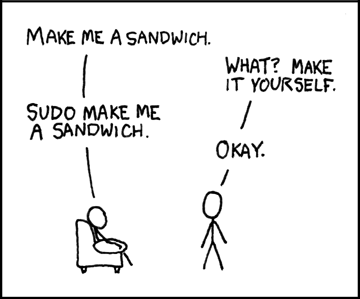
\includegraphics[width=\linewidth]{sandwich.png}
\caption{xkcd shows what-if linux was real world}
\label{fig:sandwich}
\end{marginfigure}

\subsection{Further Resources}
\newthought{As you can notice} this is very rudimentary introduction to Ubuntu's command line. If you did not have enough time to go through the commands or you did not have access to linux machine, it is fine. As we will proceed further to use \Li, we will revise the commands and what it does.\sidenote{There are many online resources available to acquaint oneself with \href{http://lifehacker.com/how-can-i-quickly-learn-terminal-commands-1494082178}{ basic ubuntu commandline}. This is also a good discussion on how to learn the \href{http://ubuntuforums.org/showthread.php?t=275446}{commands}}

Also there is available a very comprehensive \href{http://cli.learncodethehardway.org/bash_cheat_sheet.pdf}{cheatsheet or refcard } where many important commands are written in tabular form. It is recommended to go through the list and test whichever looks interesting. 



%----------------------------------------------------------------------------------------
%	CHAPTER 2
%----------------------------------------------------------------------------------------

\chapter{Working with \Li}
\label{ch:2}

\section[Introduction]{Introduction}

\begin{fullwidth}
  In this section, we will get to speed by directly diving deep into working with \Li. As \Li does not have a graphical user interface, the commands that we saw in the previous section ( see \textsc{Table} \ref{command0}, \textsc{Table} \ref{command1} and \textsc{Table} \ref{command2}).
  \end{fullwidth}


  In this section, we will do the following:
  \begin{itemize}
  \item Run example scripts of \Li
  \item Convert the results into \textit{VTK Format} using \textit{LPP.py} and understand the need for it
  \item Post Process or View the results in the \textit{Paraview} Software
  
  \end{itemize}
%----------------------------------------------------------------------------------------

 \section[Example Scripts]{Example Scripts}

 \newthought{The examples} scripts are present default in the folder:


 It can be accessed by
\begin{marginfigure}
  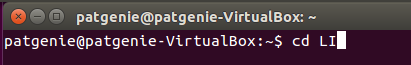
\includegraphics[width=\linewidth]{graphics/Screenshot/Lig2.png}
\caption{Typing in the terminal}
  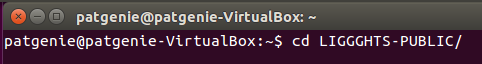
\includegraphics[width=\linewidth]{graphics/Screenshot/Lig3.png}
\caption{On pressing the TAB Command}
  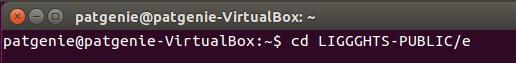
\includegraphics[width=\linewidth]{graphics/Screenshot/Lig4.png}
  \caption{Using TAB Again }
  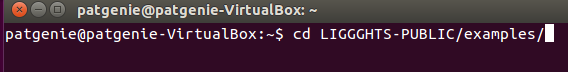
\includegraphics[width=\linewidth]{graphics/Screenshot/Lig5.png}
  \caption{Demonstration of Auto completion command}
  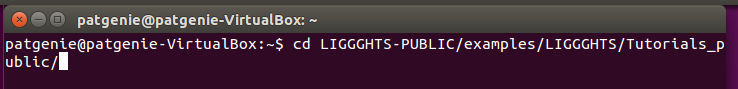
\includegraphics[width=\linewidth]{graphics/Screenshot/Lig6.png}
  \caption{Getting into Examples Folder}
  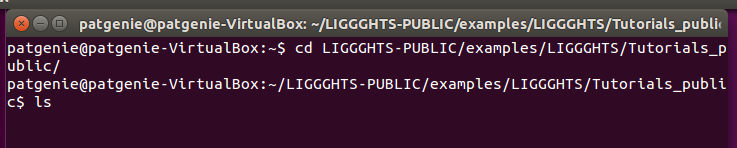
\includegraphics[width=\linewidth]{graphics/Screenshot/Lig7.png}
  \caption{Press enter}
 
  \label{fig:lig1}
\end{marginfigure}
\begin{figure}
  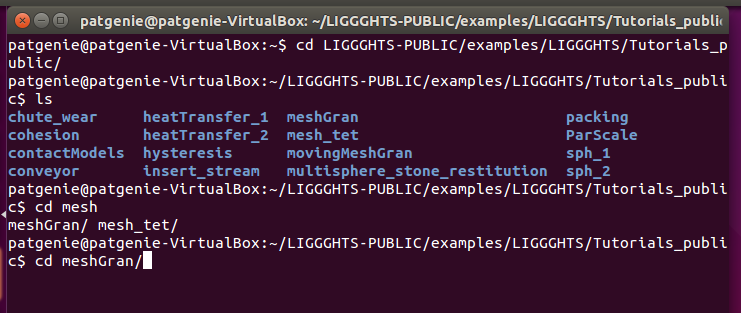
\includegraphics[width=\linewidth]{graphics/Screenshot/Lig8.png}
  \caption[-14ex]{List of example files}
  \\\vspace{\baselineskip}
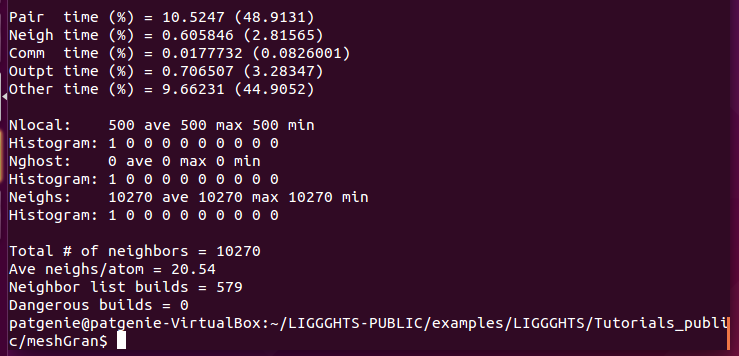
\includegraphics[width=\linewidth]{graphics/Screenshot/Lig13.png}
  \caption[-14ex]{Successfully converted all the files}
\setfloatalignment{b}
  \label{fig:lig8}
\end{figure}

\textit{All the steps are shown in the Figure \ref{fig:lig1}}
 \begin{itemize}
 \item First going to home folder using \textit{\emph{cd \~}}
 \item Then using typing \textit{\emph{cd \Li-PUBLIC}}. As mentioned earlier you use TAB Completion to save time while writing.
 \item \textit{\emph{ls}} to show the files and folders 
 \item Again type \textit{\emph{cd examples}} to change directory to examples script
 \item \textit{\emph{ls}} to show the files and folders
 \item Type \textit{\emph{cd \Li}} and \textit{\emph{cd tutorials}} to reach example scripts
   
 \item Type \textit{\emph{ls}} to show the list of examples
 \end{itemize}
 \index{Examples}
\subsection{Running \Li Script}



 In this section we will run the script of MeshGran. A \Li simulation file can be run in the following method:
\begin{itemize}
 \item In the Examples folder, change directory to the MeshGran using \textit{\emph{cd meshgran}}
 \item Type \textit{\emph{ls}} to show the contents of the folder
 \item The \textit{\emph{in.meshGran}} file is the input script for \Li simulation
 \item Run the script using \textit{\emph{liggghts < in.meshGran}}
 \item If there are any errors in the input script, the task would show the error and close out. 
 \item If there are no errors, then you should successfully written command
 \end{itemize}
\index{Input Script}
\emph{ See Figure 13, 14 \& 15 for instructions. }

 \begin{marginfigure}
   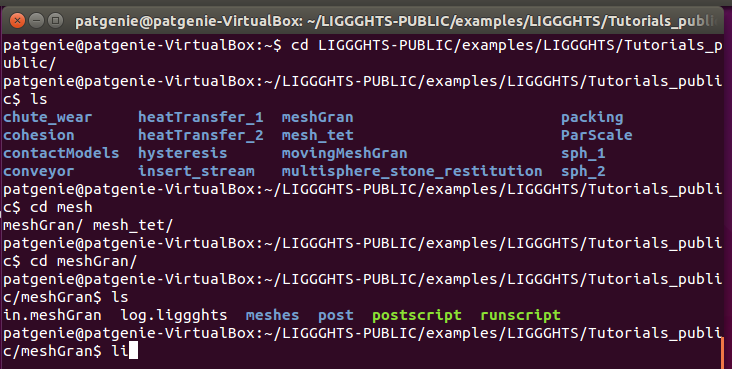
\includegraphics[width=\linewidth]{graphics/Screenshot/Lig10.png}
   \caption{Type li into the shell prompt and hit}
 \end{marginfigure}
  \begin{marginfigure}
   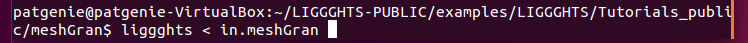
\includegraphics[width=\linewidth]{graphics/Screenshot/Lig11.png}
   \caption{Type liggghts < in.meshGran}
 \end{marginfigure}
  \begin{marginfigure}
   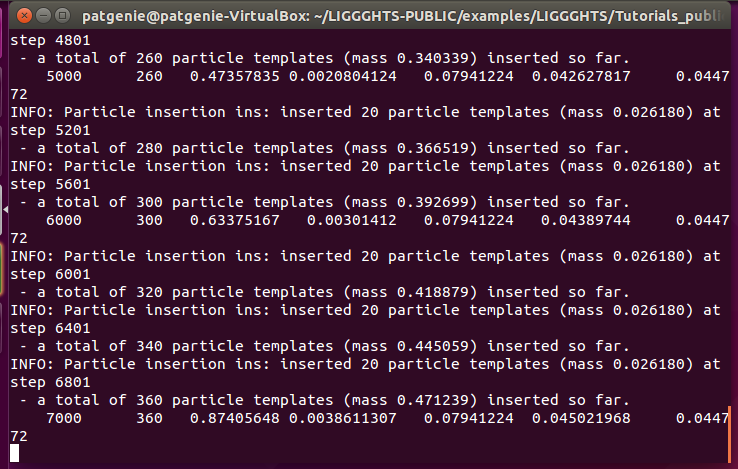
\includegraphics[width=\linewidth]{graphics/Screenshot/Lig12.png}
   \caption{\Li should begin executing the file}
 \end{marginfigure}
 \newthought{If everything} went smoothly, congratulations, you have run your first \Li script file successfully.

 \section[Converting the files]{Converting the files}
 \begin{marginfigure}
   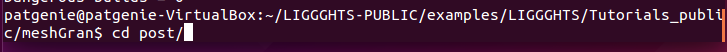
\includegraphics[width=\linewidth]{graphics/Screenshot/Con1.png}
   \caption{To view results, goto the post folder}
  
   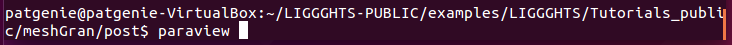
\includegraphics[width=\linewidth]{graphics/Screenshot/Con4.png}
   \caption{Type paraview, to enter paraview}
 \end{marginfigure}
 \begin{figure}
 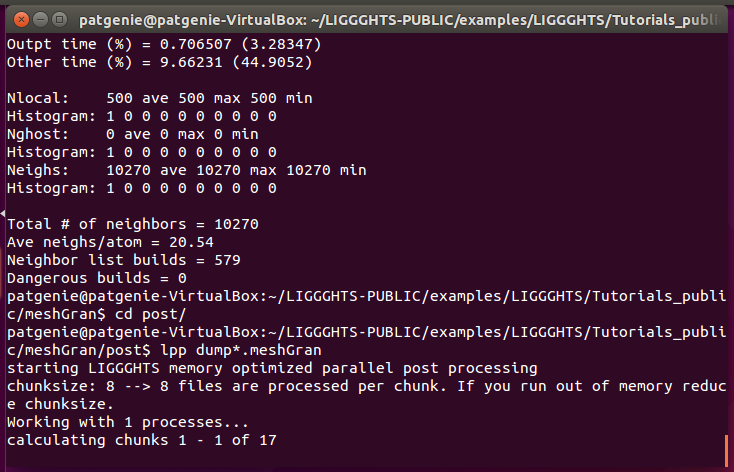
\includegraphics[width=\linewidth]{graphics/Screenshot/Con2.png}
 \caption{LPP Processing files}
 \textit{The LPP command can be started with \textbf{lpp dump*.meshGran}in the post folder of the \Li}
 \end{figure}
 \begin{fullwidth}
   \newthought{Although} we completed the running the input script file in the last section, we won't be able to see what we have done as the file generated by the \Li input file is compatible with any software. To get around this, we first need to convert the files generated to a format that we can use to visualise the results that we got. In our case, the format we use will be VTK. VTK stands for \textit{Visualisation Toolkit}
   Let us see, how we can convert the files into VTK file format
 \end{fullwidth}

 The following method should be used:
 \begin{itemize}
 \item Once the files are converted, the \Li files are usually stored in the post folder. Therefore, change directory to Post folder using command \textit{\emph{cd post}}. \textit{(See Figure 16})
 \item In the post folder, type \textit{\emph{lpp dump*.meshGran }} to convert all the timesteps generated into VTK format.
 \item Once the operation is complete, you should see it has successfully completed the operation.
 \end{itemize}
\section[Using Paraview]{Using Paraview }
 \index{Paraview}
 
 \begin{figure}
  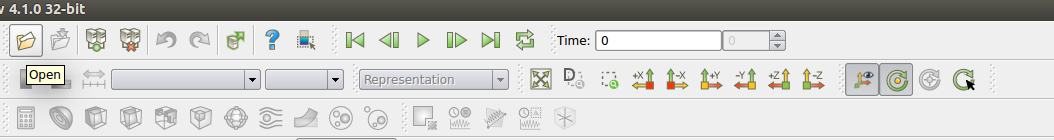
\includegraphics[width=\linewidth]{graphics/Screenshot/P1.png}
    \end{figure}
 \begin{marginfigure}
   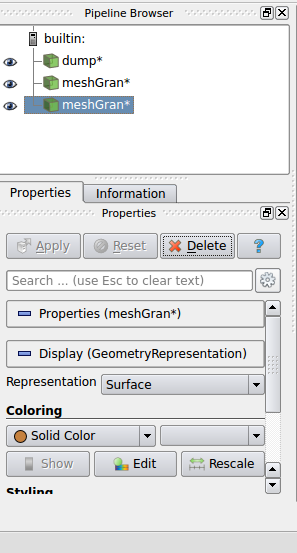
\includegraphics[width=\linewidth]{graphics/Screenshot/P3.png}
   \caption{Properties Browser}
   \vspace{3ex}
 \end{marginfigure}
 \begin{marginfigure}
   
\includegraphics[width=\linewidth]{graphics/Screenshot/P4.png}
   \caption{Playback Bar}
 \end{marginfigure}
Now that we have got the files and folders in the format that is compatible, we can view our results in the Paraview software.
\begin{figure}
  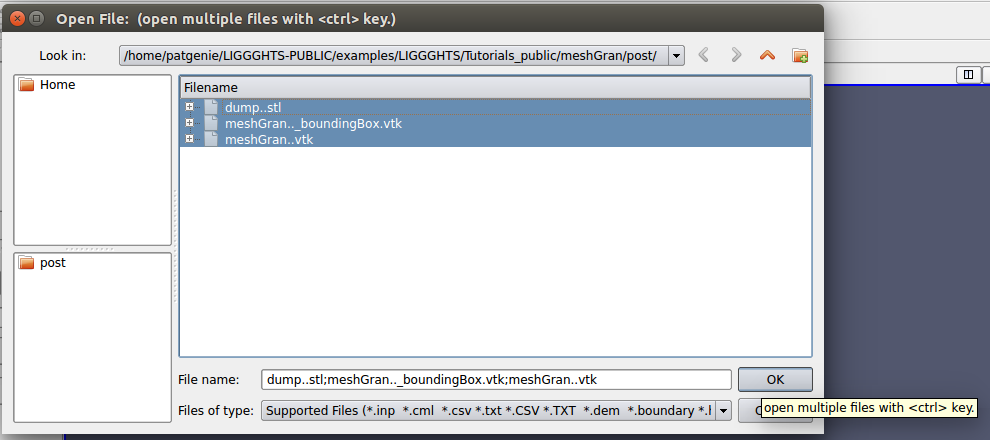
\includegraphics[width=\linewidth]{graphics/Screenshot/P2.png}
 
  
\end{figure}
\begin{figure}
  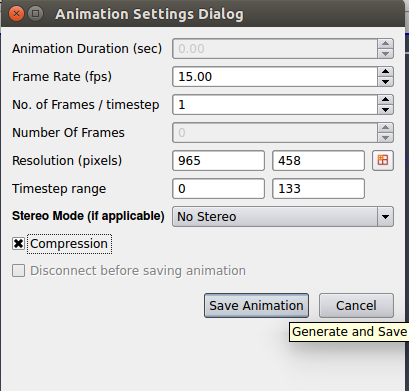
\includegraphics[width=\linewidth]{graphics/Screenshot/P5.png}
  
  \caption{Saving Animation}
  \label{fig:P5}
\end{figure}
\\\vspace{\baselineskip}

 We can enter Paraview and use it by the following method:
 \begin{itemize}
 \item Type paraview in the post folder
 \item Click on the Open Icon, and the select all.(See Figure 22)
 \item Click Apply on the property bar shown in the Figure 20.
 \item Once, the files and setting have imported into the region, you can begin by clicking on the play button on the playback bar. 
 \item You can also save the animation in \emph{File->Save Animation}
 \item You can choose the format, avi((if available)).
 
 \end{itemize}
\section{Opening the input file}

\begin{figure}
  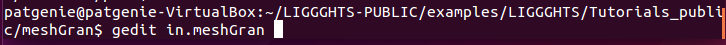
\includegraphics[width=\linewidth]{graphics/Screenshot/Gif1.png}
  \caption{Opening the file using command prompt}
  \end{figure}

\begin{figure}
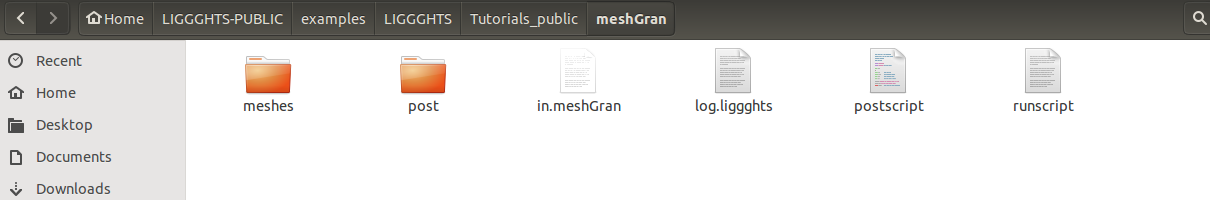
\includegraphics[width=\linewidth]{graphics/Screenshot/Gif3.png}
  \caption{Opening the files using File Manager}
\\\vspace{\baselineskip}
\end{figure}

You can open the input file using the shell prompt, as shown in the figure 24. Also you can open the file using a file manager shown in the figure 25. The default application for text editing in ubuntu is an application of \emph{Gedit}.

\section{Different Files and format }

Before delving into the file structure, there are few file formats that needs to be explained.
\marginnote{ In the meshGran folder
  \begin{itemize}
  \item \textbf{in.meshGran} is the main input script
  \item \textbf{mesh} is the folder where stl files are kept
  \item \textbf{post} is the folder where generated files are kept
  \end{itemize}
}
\begin{itemize}
\item \textbf{dump*.meshGran:} It is the dump file generated by \Li at a given timestep. All the specification that you write to dump is dumped here. We will see ahead how you can generate. The \* stands for all them. There is a dumpfile for each timestep interval. Therefore while converting in LPP, we use the asterisk(\*) as a placeholder for everyone of them.  You can open and have a look what's inside to get a better idea about this file.
\item \textbf{dump.vtk:} After running the LPP converter script, these are the output we get. These can read by Paraview. 
\item \textbf{meshGran.stl:} The stl/cad files that you import during the script are store in these scripts. unlike the .meshGran format which is unreadable by Paraview, these are perfectly readable by paraview. Like the dump files, sometimes these are also store on regular timestep interval, the idea behind being if there is motion of the stl file for e.g rotation of feedframe, the location and position should be stored somewhere to visualise it later. 
\end{itemize}
 \section{Anatomy of input file}

 \begin{fullwidth}
   \newthought{Now that} we have run an example script, we are in a good position to understand what is inside the \Li input file.
   Let us first look into the meshgran input file, for better understanding.
 \end{fullwidth}

 
   
 \inputminted{cpp}{in.meshGran}
   
  


 \newthought{The Input script} can be divided into four parts.
 \begin{itemize}
 \item \textbf{Initialisation} Setting the parameters that are needed to defined before the particles can be created. 
 \item \textbf{Properties} Defining the properties of materials, particles to be inserted, geometry, defining walls and particle generation.
 \item \textbf{Detailed Settings} Defining settings that correspond to output, the integreting method to be used etc
 \item \textbf{Execution} The actual run command that executes the simulation. 
 \end{itemize}


\subsection{Initialisation}
\marginnote{\textsc{Commands that you can alter}: \textbf{boundary, units, region, create\_box, neighbor and neigh\_modify}}


\begin{minted}{cpp}
# Define the style of atom that you would like to simulate
atom_style	granular
# Set the boundary to movable i.e as atoms cross the boundary, the boundary expands
boundary	m m m
newton		off
atom_modify	sort 0 0
communicate	single vel yes
# Set the unit system to SI units
units		si
# Define the region in space where simulation will occur
region		reg block -0.01 0.51 -0.06 0.01 -1.22 0.01  units box
# Specify the number of atoms that will be involved and the region command
create_box	1 reg

neighbor	0.02 bin
neigh_modify	delay 0

\end{minted}
\marginnote{\textsc{Commands that is best left as it is unless you know what you are doing}: \textbf{atom\_style, newton, atom\_modify}}

\subsection{Properties}

\begin{minted}{cpp}
  /*Material properties required for new pair styles. Notice the format is
  same for all the properties. It shows the important properties required
  for a basic granular simulation.*/

fix 		m1 all property/global youngsModulus peratomtype 5.e6
fix 		m2 all property/global poissonsRatio peratomtype 0.45
fix 		m3 all property/global coefficientRestitution peratomtypepair 1 0.7
fix 		m4 all property/global coefficientFriction peratomtypepair 1 0.05
fix 		m5 all property/global characteristicVelocity scalar 2.

/* Import triangular mesh from a cad file. It can scaled, moved and rotated */
fix		cad all mesh/surface file meshes/mesh.stl type 1 scale 0.001 &
                move 0. 0. 0. rotate axis 1. 0. 0. angle -90.

/* We will use the previously imported mesh as a wall */
fix             granwalls all wall/gran model hooke tangential history mesh &
                n_meshes 1 meshes cad

/* We can insert particles by defining an insertion face.
This can be done by either importing a cad file and using
it as insertion face or using primitive shapes from \Li library*/
fix		inface all mesh/surface file meshes/insertion_face.stl type 1

#Define a basic template of a particle to be inserted
fix		pts1 all particletemplate/sphere 1 atom_type 1 density constant 2500 radius constant 0.005
# Using the template defined previously, create distribution
fix		pdd1 all particledistribution/discrete 1.  1 pts1 1.0
#Group the particles together
group		nve_group region reg

/*Now the insert the particles using distribution template and insertion face
defined earlier. We can also give addition info such as velocity.
We can insert the particles using mass, volume or number. */
fix		ins nve_group insert/stream seed 5330 distributiontemplate pdd1 &
                maxattempt 100 nparticles 10000 particlerate 1000 overlapcheck yes&
                all_in no vel constant 0. 0. -1.0 &
	        insertion_face inface extrude_length 0.02

#New pair style
pair_style gran model hooke tangential history /*Hooke without cohesion*/
pair_coeff * *
\end{minted}
\marginnote{Here the important thing to understand is you don't have to understand everything. Here is a very high level overview to understand the input file. However, while making your own script, you will mostly be tweaking these parameters/settings. }

\subsection{Detailed Settings}
\marginnote{Very rarely you would need to change these settings}
\begin{minted}{cpp}
/* Define the timestep equal to 0.001 sec.
    The unit depends on the SI unit used.
    It is recommended that the simulation should
    be 20\% or lesser than a Rayleigh TimeStep*/  
timestep	0.00005

/* Define the timestep equal to 0.001 sec.
    The unit depends on the SI unit used.
    It is recommended that the simulation should
    be 20\% or lesser than a Rayleigh TimeStep*/
    fix		1 all nve/sphere

/* For every particle, we define a property gravity
  acts in the direction of the vector specified */
 fix		2 all gravity 9.81 vector 0.0 0.0 -1.0

 /* Check the time step and compare it with Rayleigh.
  Give error if its greater than 0.01 \% greater.
  Initialize dump by running 1 timestep. Is recomended to do so.
  Unfix the checking after once. The result is written in log file*/
 fix		ts all check/timestep/gran 1000 0.1 0.1

/* Compute the rotational properties of sphere */
compute		1 all erotate/sphere

/*Describe quantities to be printed on logfile
  and the output screen. The number of interval to the
  write the thermodynamic quantities.
  Lost _Ignore ignore lost particle */
thermo_style	custom step atoms ke c_1 f_ts[1] f_ts[2] vol
thermo		1000
thermo_modify	lost ignore norm no
compute_modify	thermo_temp dynamic yes

/*Generates a set of dump files
  that contain information for imaging
  the system. Give the interval and file type to save.
  This generates huge files, therefore it is
  recommended to dump properties that are necessary.  */
  
dump		dmp all custom 300 post/dump*.meshGran id type type x y z  radius
dump 		dmpstl all mesh/stl 300 post/dump*.stl

\end{minted}
\vspace*{5ex}
\subsection{Execution Commands}

\marginnote{These commands are final commands, which brings the input script into action. The 10000 number is the \textit{number of Timesteps}. Considering we took timestep \textit{\emph{0.00005}} The number of seconds in the real world would be numberOfTimeSteps x TimeStep = 0.5 seconds}
\begin{minted}{cpp}
#insert particles
run			10000 upto
/*Unfix the insertion i.e stop the insertion */
unfix		ins

#run
run			40000 upto

  \end{minted}

  \subsection{Summary}

\newthought{This was an example script} that was provided in with \Li. Similar to mesh Gran example, there are a lot of different examples currently in the the examples folder of the \Li. It is recommended that the reader must at least familiarise with most of them, by simulating and reading the source code and understanding. Understandably there are many commands that one who is not familar with \Li will be able to understand . In that case, the reader should visit and look up the \href{http://www.cfdem.com/media/DEM/docu/Manual.html}{reference manual}.\sidenote{The \Li reference manual is an exhaustive manual with all the possible commands. It is not possible to read the entire manual and it is not recommended to attempt so. However, it is advisable to read the sections which where introduced in this particular chapter.}

\subsection{Exercises}

The following exercise can be done after this particular chapter to become much familiar with the material introduced in the chapter.
\begin{enumerate}
\item Run all the example scripts accompanied with LIGGGHTS.
\item Tweak parameters and notice the effect in the simulation: \textbf{radius, run, disable the unfix, boundary, units }   

\end{enumerate}
  
%----------------------------------------------------------------------------------------
%	CHAPTER 3
%----------------------------------------------------------------------------------------

\chapter[Making your own Simulation]{Making your own simulation}
\label{chap:3}

\begin{fullwidth}
The most important part of this documentation is how you can go on and design your own simulation using \Li. In the chapter we will go over some of the steps that will enable you to do that.
  
\end{fullwidth}

\section{Pre-requisites}

There are few pre-requisite or preliminary data that needs to be collected before creating a \Li Simulation. The following constitutes the
\begin{itemize}
\item \textbf{Number of Different Atoms}
  In \Li, walls are basically composed of atoms/particles. The properties assigned to these atoms acts for the wall as well. Therefore if you will working with, lets say three powder, the number of different atoms will be \textit{3 + 1 = 4}
\item \textbf{Radius of each particle size} The size of particles. Either a constant value or a Gaussian Value with Standard Deviation and Mean size.
\item\textbf{ Density of particles} The true density of particles. Similar to the radius, either a constant value or a Gaussian Value with SD and Mean size.
\item \textbf{Coefficient of Friction} The Coefficient of friction requires symmetric matrix, with combination of different particles with each other.
  \begin{figure}
    \centering
    $COF =
    \begin{bmatrix}
      P_{11}&P_{12}&P_{13}\\ P_{21}&P_{22}&P_{23} \\
      P_{31}&P_{32}&P_{33}
   
    \end{bmatrix}$
     
    
    \caption{Symmetric Matrix}
    \label{fig:matrix}
  \end{figure}
 \marginnote{ COF is a symmetric matrix as$ P_{ab} = P_{ba}$ for the coefficient of friction between two particles.}
\item \textbf{Coefficient of Restitution} The Coefficient of Restitution also requires a symmetric matrix, with the combination of different particles with each other.
\item \textbf{Poisson's Ratio} A constant value for each particle.
\item \textbf{Young's Modulus} A constant value for each particle.
\item \textbf{Cohesion or No Cohesion} In case using cohesion, then the value of Cohesion Energy Density is required.
\item\textbf{ The CAD File} and the\textbf{ dimensions} and orientations are needed to properly set up.
\item \textbf{The Domain box} It is the region where the simulation will occur. It is an imaginary control volume in space, in which all the particles and geometry is kept. If the particles go out of the domain box, then the simulation stops, unless specified to ignore lost particles. The \textbf{\emph{boundary}} command sets up the dimension of the domain box. It should be noted that this should be minimum as possible and should completely engulf the geometry. If you have a system where the atoms will move past the boundary, then it is recommended to have the domain be movable. 
\end{itemize}

\section{Steps Involved}
\begin{fullwidth}
  \newthought{Now that you } have all the information, we can move along to create our own first simulation. In this particular section we will re-construct the feedframe and understand, how one might do so from scratch. 
\end{fullwidth}

\begin{itemize}
\item Define your objective
\item Setting up meshing and domain box
\item Collecting Particle Properties information
\item Write the Initialization Part
\item Write the Properties Setup
\item Write the Detailed Settings
\item Write the Execution and further Settings
\end{itemize}

\textit{We will walkthrough all of that using the following two settings. Next Stop. \textbf{The FeedFRAME Junction} }

\section{The Tale of FeedFrame}

Feedframe is a part of tab-letting process in the drug-manufacturing process of pharmaceutical industries. Our goal here will be emulate the behaviour of feedframe with a binary mixtures ( in our case beads ), and make note of the segregation tendencies that results.

   \begin{marginfigure}
   \fbox{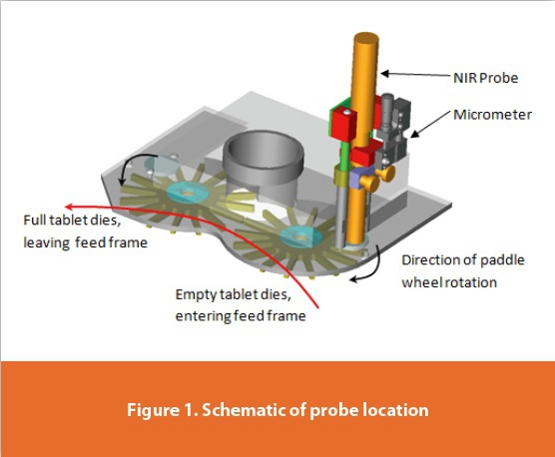
\includegraphics[width=\linewidth]{graphics/feedframe.jpg}}
   \caption{Graphical Representation of feedframe.Image taken from the \href{http://www.americanpharmaceuticalreview.com/Featured-Articles/116357-Sample-Presentation-in-Rotary-Tablet-Press-Feed-Frame-Monitoring-by-Near-Infrared-Spectroscopy/}{paper} }
 \end{marginfigure}

\subsection{Defining our objective}

We will have the following objectives.
\begin{itemize}
\item Filling the feedFrame with beads uniformly
\item Rotating the feedframe with some angular velocity to check their effect
\end{itemize}

\subsection{Setting up the meshing and domain box}

Once we have defined our objective, we can now work towards where we will fill the particles. That requires to first examine our geometry that we have and construct an insertion face.
\begin{figure}
  
\fbox{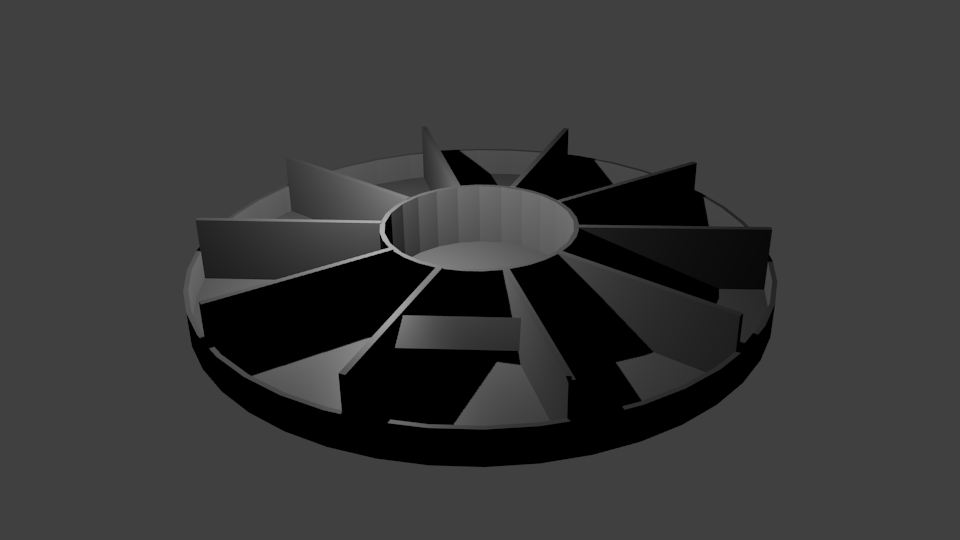
\includegraphics[width=\linewidth]{graphics/Object/MainView.png}}
  \caption{Main View}
  \label{MainView}
\end{figure}
\begin{figure}
  
\fbox{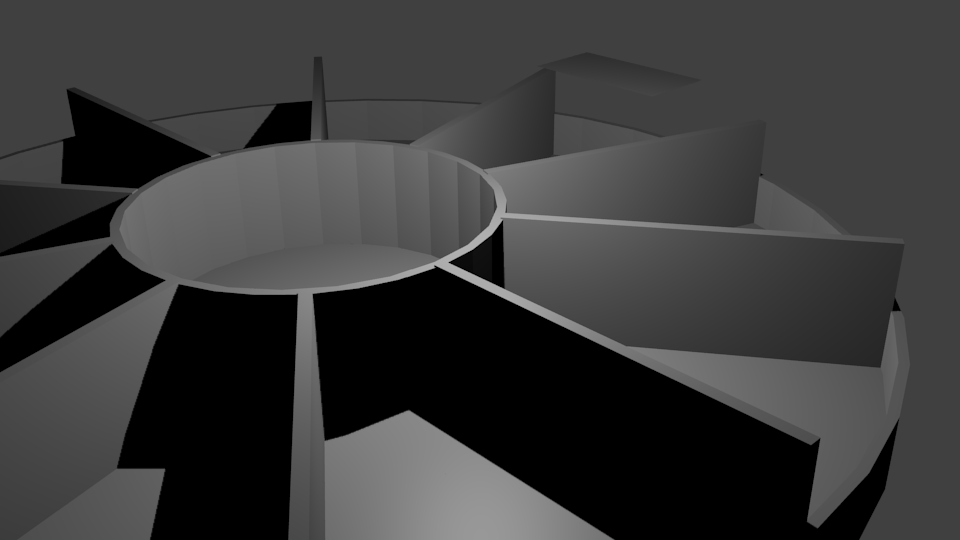
\includegraphics[width=\linewidth]{graphics/Object/SideView.png}}
  \caption{Side View}
  \label{SideView}
\end{figure}\begin{figure}
  
\fbox{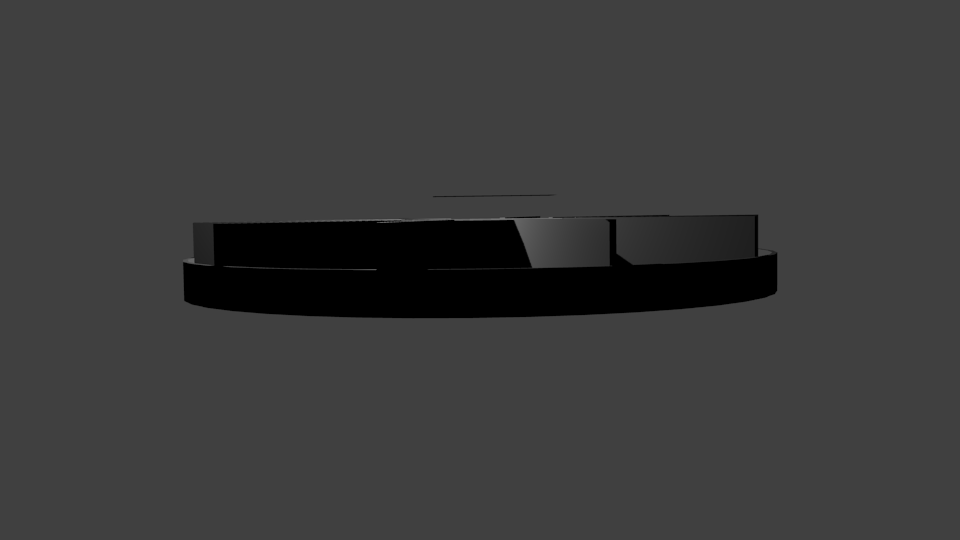
\includegraphics[width=\linewidth]{graphics/Object/Side2View.png}}
  \caption{Another Side View}
  \label{Side2View}
\end{figure}

In the Figure \ref{MainView}, \ref{SideView} and \ref{Side2View}, we can see three objects.
There is the \textbf{outer base, an inner paddle} and a \textbf{rectangle face} just right up top of a paddle.

The rectangle face will act as our insertion face i.e the region from where the particles will generated and dropped into the simulation box.

\newthought{The whole setup } was created in blender, which is an excellent open source free software for \textit{Modelling, Meshing, Rendering, Visualising} and lots more. This documentation wouldn't cover CAD Modelling, however there are tons of resources online, which can you get you started working on it.

The important thing to remember is the following:
\begin{itemize}
\item The geometry should be at the origin
\item The relative position of multiple geometries should be carefully noted.
\item The dimensions of the geometry should be noted.
\end{itemize}

The geometry should be at origin because, \Li is completely based on commandline. As there are no GUI available, it is often difficult to get an idea where our imported geometry is. Keeping the geometry to origin makes sure that our geometry land right at the origin.

The following are the dimensions obtained:
\begin{table}
  \centering
  \begin{tabular}{ll}
    \toprule
     Direction &  Highest Magnitude \\
    \midrule
     \textbf{X} & 24 \\
    \textbf{Y} & 24 \\
    \textbf{Z} & 3.5 \\
    \bottomrule
  \end{tabular}
  \caption{Dimension Info}
  
  \label{tab:dimensions}
\end{table}
\marginnote{There are no dimension associated with an stl file. It is usually set by the \textit{Units} command in \Li. Therefore we will have \textit{24 m} for an SI unit while \textit{24 cm} for CGS}

\subsection{Collecting particle properties information}
\begin{table} % Add the following just after the closing bracket on this line to specify a position for the table on the page: [h], [t], [b] or [p] - these mean: here, top, bottom and on a separate page, respectively
\centering % Centers the table on the page, comment out to left-justify
\begin{tabular}{l c c c} % The final bracket specifies the number of columns in the table along with left and right borders which are specified using vertical bars (|); each column can be left, right or center-justified using l, r or c. To specify a precise width, use p{width}, e.g. p{5cm}
\toprule % Top horizontal line
& \multicolumn{3}{c}{Properties of Particles} \\ % Amalgamating several columns into one cell is done using the \multicolumn command as seen on this line
\cmidrule(l){2-4} % Horizontal line spanning less than the full width of the table - you can add (r) or (l) just before the opening curly bracket to shorten the rule on the left or right side
Properties Name & $P_1$ & $P_2$ & Wall \\ % Column names row
\midrule % In-table horizontal line
Young's Modulus & $5X10^7$ & $5X10^7$ & $5X10^7$ \\ % Content row 2
  Poissons Ratio & 0.45 & 0.45 & 0.50 \\ % Content row 3
  Radius & 0.001 & 0.001 & 0.001 \\
  Density & 7800 & 1190 & 2000 \\
\midrule % In-table horizontal line

\bottomrule % Bottom horizontal line
\end{tabular}
\caption{Properties Table} % Table caption, can be commented out if no caption is required
\label{tab:template} % A label for referencing this table elsewhere, references are used in text as \ref{label}
\end{table}

 \begin{marginfigure}
    \centering
    $COF =
    \begin{bmatrix}
      0.7&0.65&0.68\\ 0.65&0.60&0.68 \\
      0.68&0.68&0.3
   
    \end{bmatrix}$
\vspace{2ex}
    $COR =
     \begin{bmatrix}
      0.25&0.24&0.23\\ 0.24&0.35&0.23 \\
      0.23&0.23&0.22
   
    \end{bmatrix}$
    
    \caption{Coefficient of Restitutions and Friction}
    \label{fig:matrix}
  \end{marginfigure}

\subsection{Writing the Initialisation}
\begin{minted}{cpp}
  /*Initialisation*/
  atom_style   granular
  atom_modify  map array
  boundary     f f f
  newton       off
  /*processors  1 1 2 This is commented as the we are
  not using parallel processing */

  communicate  single vel yes

  units        si

  /* cylinder args = dim c1 c2 radius lo hi
      dim = x or y or z = axis of cylinder
      c1,c2 = coords of cylinder axis in other 2 dimensions (distance units)
      radius = cylinder radius (distance units)
      radius can be a variable (see below)
      lo,hi = bounds of cylinder in dim (distance units)

      region void cylinder y 2 3 5 -5.0 EDGE units box*/
  region       reg cylinder z 0 0 0.125 -0.03 0.08 units box 

  create_box   3 reg

  neighbor     0.001 bin

  neigh_modify delay 0
  
\end{minted}
\marginnote{For more information on how to setup the region, visit \href{http://www.cfdem.com/media/DEM/docu/region.html}{here} } 
The following needs to written during the initialisation. These commands are not needed to be remembered. You can copy off from an example file and edit on your own.
\begin{itemize}
\item \textit{Boundary} The rational behind making boundary fixed is so that we know if a geometry is getting out of the domain box or the particle is getting out of domain box.
\item \textit{Region} Since, we are using a cylindrical system, it is best to use a cylindrical shaped domain box. This would result is less empty space, hence saving in computation. 
\item \textit{Create\_Box} We will use 3 atoms and the domain is the cylinder we just specified
\item \textit{Neighbor} The neighbour list will be created at a distance which is approximately equal to the diameter of the atom.
\end{itemize}

\subsection{Writing the Properties}
The following are the properties that will needed to be written 
\begin{itemize}
\item Material properties \textit{for example young's modulus, friction etc}
\item Importing Geometries to be used as wall and using the imported geometries as wall
\item Insertion face
\item Particle template
\item Particle distribution template
\item Particle insertion 
\item Pair style
\item Gravity
\end{itemize}

\begin{minted}{cpp}
# Properties of Material

fix 		m1 all property/global youngsModulus peratomtype 5.e7 5.e7 5.e7
fix 		m2 all property/global poissonsRatio peratomtype 0.45 0.45 0.50 
fix 		m3 all property/global coefficientFriction peratomtypepair &
                3 0.7 0.65 0.68 0.65 0.60 0.68 0.68 0.68 0.3
fix 		m4 all property/global coefficientRestitution peratomtypepair &
                3 0.25 0.24 0.23 0.24 0.35 0.23 0.23 0.23 0.22
  \end{minted}
  \textbf{Properties Setting}
  The setting of properties is pretty much self explanatory. For every peratomtype, you would need input values for each material type. For every peratompair properties, you would need to give the matrix in the form of Figure \ref{fig:matrix}
  \begin{minted}{cpp}
    /* Importing Geometries */
   
fix		out all mesh/surface file mesh/OuterPaddle.stl type 3 scale 0.01
fix		incad all mesh/surface file mesh/InnerPaddle.stl type 3 scale 0.01&                curvature 1e-5 
# Make the imported cad as walls 
fix 		wall all wall/gran model hertz tangential history mesh &
                n_meshes 2 meshes incad out
  \end{minted}
  \begin{itemize}
  \item \textbf{file} keyword refers to a location of file 
  \item \textbf{Type} refers to the atom type. We will refer all the walls being consist of a atom of type 3
  \item \textbf{Scale} It can be seen that the dimensions if used directly will be enormous. For \textit{example} 24 m. Therefore we will scale down our imported geometry down 100 times. 
  \item \textbf{Wall/gran} This command converts the imported geometry to walls.

  \end{itemize}
  
  \begin{minted}{cpp}
# use the walls to fix the domain box with primitive walls
fix 		zwalls1 all wall/gran model hertz tangential history &
                primitive type 3 zcylinder 0.125 0 0
#Use the wall at the time of filling
fix 		cylinder1 all wall/gran model hertz tangential history &
                primitive type 3 zcylinder 0.12 0. 0. 
fix 		cylinder2 all wall/gran model hertz tangential history &
                primitive type 3 zcylinder 0.04 0. 0. 

# region for insertion
fix 		inface all mesh/surface file mesh/insertionFace.stl type 3 scale 0.01


\end{minted}
Apart from the traditional imported walls, we can also generate walls within \Li itself. This is done by using the primitive type command. \sidenote{For more information, visit \href{http://www.cfdem.com/media/DEM/docu/fix_wall_gran.html}{here}}
The insertion face can be imported using the similar command as of geometry. Notice the type and scale keywords.
\begin{minted}{cpp}
  /* distributions for insertion */
  fix		pts1 all particletemplate/sphere 1 atom_type 1 &
                density constant 7800 radius constant 0.00100
  fix		pts2 all particletemplate/sphere 1 atom_type 2 &
                density constant 1190 radius constant 0.00100
  fix		pdd1 all particledistribution/discrete 1.  2 &
                pts1 0.50 pts2 0.50



              \end{minted}
In this particular step, we did two things
\begin{itemize}
\item Defined the basic template of particles i.e \textit{radius, density and atom type}. It is always good practice to define different atom types with different type of atom. Currently you can define upto 32 atoms of atoms.
\item Defined the distribution of the insertion. Here we are taking 50 \% of particle 1 and \% of particle 2 in the distribution. Thus it is a perfectly homogenous mixture distribution.
\end{itemize}

\begin{minted}{cpp}
/* particle insertion */
fix         ins all insert/stream seed 1001 distributiontemplate pdd1 &
            nparticles 6000 vel constant 0. 0. -0.2. particlerate 20000 &
            overlapcheck yes insertion_face inface extrude_length 0.015                
\end{minted}
\textbf{Particle Insert Stream} The Latest version of \Li, which as of now is 3.3.0, offers some really great optimisations in the insertion using insert/stream method.
\begin{itemize}
\item \textbf{Seed} This is a random number generator, to make the simulation for more non-deterministic.
\item \textbf{Distribution Template} This is the Distribution we just defined with perfectly homogenous mixture.
\item \textbf{nparticles} We will use the number of particles method. 
\item \textbf{vel constant} We can use the velocity at the time of insertion. The input here is a vector. This one points that it will have \textit{0.2 metres/sec} in the negative z direction. 
\item \textbf{Insertion Face} The geometry we had imported earlier to be used as insertion face. 
\item \textbf{Extrude length} The commands extrudes the planar insertion face to create a region, from where particles will be generated. 
\end{itemize}

\begin{minted}{cpp}
  /* New pair style */
pair_style      gran model hertz tangential history # Hertzian without cohesion
pair_coeff	* *

  /*Timestep */
timestep	0.00001

/* Defining 
fix		2 all gravity 9.81 vector 0.0 0.0 -1.0

\end{minted}

\textbf{Pair Style}
In general, \Li provide two pair styling.
\begin{itemize}
\item Hooke
\item Hertz
\end{itemize}
Hertz performs better for short range forces and therefore we will use that for our granular simulation. \sidenote{You can find out more about it \href{http://www.cfdem.com/media/DEM/docu/pair_gran.html}{here}}
The \textit{pair style * *} commands refers that all atom type interaction interaction follows the same pairing defined by the hertz. We can also define separate pair for interaction of two different atoms here. If we need to add cohesion into our system, then we can write
\begin{minted}{cpp}
  pair_style gran model hertz tangential no_history cohesion sjkr 
\end{minted}
\sidenote{For more information on cohesion, you can find \href{http://www.cfdem.com/media/DEM/docu/Section_gran_models.html}{here}}

\textbf{Timestep} It is generally advised to have a timestep about 20 \% of the Rayleigh timestep. You can check the hertz time being
$$ Rayleigh Time Step =  \frac{R\times\pi\times\sqrt{\rho/G}}{(0.1631\times\nu + 0.8766)} $$
\marginnote{Here, $\rho$ is density, G is Youngs Modulus, $\nu$ is poissons ratio and R is the radius}

The first thing to determine the time step will be to calculate the Rayleigh timestep and take around 20\% of its value. Other wise, you could use an inbuilt function of \Li to use an inbuilt function to calculate the Rayleigh timestep and adust your timestep accordingly.


\begin{minted}{cpp}
/* Detailed Settings */
#apply nve integration to all particles that are inserted as single particles
fix		integr all nve/sphere

/* output settings, include total thermal energy */
fix		ts all check/timestep/gran 1000 0.1 0.1
compute		1 all erotate/sphere
thermo_style	custom step atoms c_1 f_ts[1] f_ts[2]  
thermo		1000
thermo_modify	lost ignore norm no
compute_modify	thermo_temp dynamic yes


\end{minted}

 Calculations and thermodynamic properties.
 
The thermostyle command is actually the log output and terminal that you see during the operation of \Li. Here we can see that we will observe the number of steps, number of atoms, the rotational energies and the Rayleigh and Hertz Time.
\begin{minted}{cpp}

/* insert the first particles so that dump is not empty */
run			1
dump		dmp all custom 100 post/dump*.feedFrame id type type x y z ix iy iz vx vy vz radius density  
dump 		dmpstl all mesh/stl 100 post/dump*.stl

#insert particles
run		40000 upto
unfix		ins
fix 		move all move/mesh mesh incad rotate origin &
                0. 0. 0. axis  0. 0. 1. period 10
run 		100000 upto 

\end{minted}
It is highly recommended that we should run 1 simulation first, so that the first timeslot is not null.
The dump commands generate dump files.
As we had the insertion, running will insert until we run out of timesteps or particles to insert. Once we are satisfied  that we have inserted all the particles or we want to stop the insertion in the midst, we can unfix the ins.

The second fix command, actually starts rotating the mesh around the origin and it rotates upto 100000 timesteps. In this case, the incad or the inner paddle is rotated. We can also rotate, the outer paddle and it will be the exact same thing. 

\section{Errors, Errors Everywhere}
The first time you will run your own manufactured code, there is high chances that you will get an error. But do not worry, errors are handled pretty well by \Li. If you have an error, then \Li will give you most information to find and debug it. The subsequent section gives some overview how to what kind of errors, one might face.
\subsection{Errors}
\begin{itemize}
\item \textbf{ERROR on proc 0: Cannot open mesh file meshes/OuterPaddle.stl (../input\_mesh\_tri.cpp:94)} Check the path given to importing mesh file
\item\textbf{ERROR: Fix wall/gran (id wall): could not find fix mesh id you provided (../fix\_wall\_gran.cpp:264)} While making the imported CAD as walls, make sure that you give the correct ID, you had given while importing.
\item \textbf{ERROR: Could not find fix group ID (../modify.cpp:754)} You have given an invalid group ID.
\item \textbf{ERROR: Fix insert/rate/region (id ins1): region ID does not exist (../fix\_insert\_pack.cpp:86) If you are using an imported mesh as insertion face then rather than \textit{region}, you have to use \textit{insertion\_face} command.
11
}
  \item \textbf{ERROR: Could not locate a fix/property storing value(s) for coefficientRestitution as requested by model hertz}. (../modify\_liggghts.cpp:346)
  
\subsection{Debugging basics}

Which line prompted the error. In the process of debugging, this is the most vital question that one may ask. And \Li reads the input the file, line by line. This is a good thing for us as it will tremendously useful for us to debug it. One of the important method you could use to debug, is introducing a foreign word or an unrecognised word into the script which is bound to make it fail. This would help us narrow down to the region where there is an error.

For example consider this,

\begin{minted}{cpp}
  /*continued from previous script... */
  #output settings, include total thermal energy
fix		ts all check/timestep/gran 1000 0.1 0.1
compute		1 all erotate/sphere
thermo_style	custom step atoms c_1 f_ts[1] f_ts[2]  
thermo		1000
thermo_modify	lost ignore norm nope
compute_modify	thermo_temp dynamic ye
  \end{minted}
\end{itemize}

Running the script will give us the following error
\begin{minted}{bash}
  ERROR: Illegal thermo_modify command (../thermo.cpp:471)
\end{minted}
In order to identify where is the error, we will introduce the word \textbf{stop} somewhere in the code.
\begin{minted}{cpp}
  /*continued from previous script... */
  #output settings, include total thermal energy
fix		ts all check/timestep/gran 1000 0.1 0.1
compute		1 all erotate/sphere
thermo_style	custom step atoms c_1 f_ts[1] f_ts[2]  
stop
thermo		1000
thermo_modify	lost ignore norm nope
compute_modify	thermo_temp dynamic ye
  \end{minted}

Now running the code again, will result in the following error.

\begin{minted}{cpp}
  ERROR: Unknown command: stop (../input.cpp:256)

\end{minted}
This will give us an idea that the error is probably after the line where have put the word \textit{stop}.
\begin{minted}{cpp}
  /*continued from previous script... */
  #output settings, include total thermal energy
fix		ts all check/timestep/gran 1000 0.1 0.1
compute		1 all erotate/sphere
thermo_style	custom step atoms c_1 f_ts[1] f_ts[2]  
thermo		1000
thermo_modify	lost ignore norm nope
compute_modify	thermo_temp dynamic ye
stop
  \end{minted}

Running the code again results in
\begin{minted}{bash}
  ERROR: Illegal thermo_modify command (../thermo.cpp:471)
\end{minted}

So, we are back to where we started. But the idea is that we know the error is amongst the two lines. And I can very well see that the keyword for \textbf{thermo\_modify} will \emph{no} instead of \textit{nope}. And that's how we catch an error.

However, you could have easily inferred that there was something wrong with thermo command from the error itself. This would not be the case everytime. Hope you get the idea.

\subsection{How to get help}

Okay, now we understand how to detect errors. The obvious next step would be debug and remove the error is to remove it. The way to do that is by refering more information on that particular command which is causing error in the \href{http://www.cfdem.com/media/DEM/docu/Section_commands.html#comm}{documentation of \Li.}
And the second place where you could get help is the \href{http://www.cfdem.com/forum}{forum}. The thing to remember is before asking any questions, you should check out previous queries by searching. There is quite less activity however the community is friendly and someone always answers your question.

\section{Summary}

Hopefully this part will make you more confident in approaching towards making your own simulation.

\chapter{Further Resources \& Ending Note}
\label{chap:4}

\begin{fullwidth}
  \newthought{Learning to work with \Li} will need much more than reading a documentation. This documentation is an attempt to initiate you with the basic skills to get you started with it. I hope that reading and working out the manual was a painless ordeal for you.  
\end{fullwidth}

\section{More functionality}
\begin{enumerate}
\item \textbf{ave/spatial:} Divides the region into bins and calculates the number of particles and their properties in each bin. Used for averaging. It can be used to calculate the \textit{Danckwert's Segregation Intensity}.
\item \textbf{property/atom/tracer: } Particles are marked if they are inside a region specified by the region\_mark keyword. Can be combined with \textbf{compute nparticles/tracer/region} to calculate the \textbf{residence time distribution} in case of a hopper.
\item \textbf{multisphere: } Treat one or more sets of atoms as independent rigid bodies.
\item \textbf{heat/gran/conduction :} Calculates the heat conduction between particles in contact.
\item \textbf{humiidity model :} LIGGGHTS can be coupled with other systems to check the effect of Water(Humidity) on the system.
\item \textbf{cohesion : } There are two models of cohesion that can be added to LIGGGHTS to simulate cohesive behaviour of substances
\end{enumerate}

\section{Further Studying}
\marginnote{The Feedframe simulation input and mesh files are accompanied with this document.}
Here is the list of further resources for you to study (\textit{if interested}) on Discrete Element Method.
\begin{itemize}
\item \href{http://www.cfdem.com/media/DEM/docu/Manual.html}{LIGGGHTS User Manual}
  It gives the most comprehensive functionalists associated with LIGGGHTS. I would recommend reading it atleast once, even though you might not understand everything at first.

\item \href{https://yade-dem.org/doc/formulation.html}{DEM Primer on Yade}
  Yade is another open source discrete element method, completely built with Python and possibly Cython. It has a good primer on DEM Formulation. 
\item \href{http://www.cimne.com/cvdata/cntr2/spc31/dtos/img/mdia/thesis/CarlesBosch.pdf}{Carles Bosch Padro\'s thesis on Discrete element simulations with \Li}
  This document specifies how \Li implements Discrete Element Method and also has a short section on DEM Theory. 
\item \href{www.springer.com/us/book/9783540214854}{Computational Granular Dynamics: Models and Algorithms}
  An excellent book defining DEM and how to implement it. It contains codes in C++ implementing the same. A definite book if you really want to learn to implement your own DEM or develop \Li or \La source code. The source code files are available in the website too. 
\end{itemize}

\section{Rationale behind working with \LaTeX}
\marginnote{Git is a powerful version control system. It stores snapshots of your current work as a set of files and the changes made to each file over time. It is a good workflow to add git in your current working directory, if your are working on a computational project. You can learn more about git \href{https://www.quora.com/What-is-git-and-why-should-I-use-it}{in a Quora answer} }

DEM is an extremely handy tool for gaining a good insight on the flow of powders. Understandably simulation of physical phenomenon is as accurate to begin with, but still can provide several results that may increase our understanding and aid us in developing appropriate models. These are the fewer incentives why you should invest in learning DEM:
\begin{itemize}
\item The models which depict real world phenomenon will become more and more accurate in the future. 
\item The cheaper computational cost will enable to calculate and host a wide range of experiments and thus gain an admirable advantage
\item Modelling flow of powders is quite difficult only through experimental calculations. Also the overhead cost and time, to model a new experimental data is quite large sometimes. 
\end{itemize}


Learning \& working with\Li would be a continual process. This documentation could serve as a basis of recording progress in the continual improvement, where new methods and algorithm implementation in \Li could be kept and added for future reference. Therefore, this documentation is available at Github repo. You are welcome fork, push changes or file issues.


%----------------------------------------------------------------------------------------
%	BIBLIOGRAPHY
% -------------------------------------------------------------------
 ---------------------

\bibliography{bibliography} % Use the bibliography.bib file for the bibliography
\bibliographystyle{plainnat} % Use the plainnat style of referencing

%----------------------------------------------------------------------------------------

\printindex % Print the index at the very end of the document

\end{document}